%%%%%%%%%%%%%%%%%%%%%%%%%%%%%%%%%%%%%%%%%
% Short Sectioned Assignment
% LaTeX Template
% Version 1.0 (5/5/12)
%
% This template has been downloaded from:
% http://www.LaTeXTemplates.com
%
% Original author:
% Frits Wenneker (http://www.howtotex.com)
%
% License:
% CC BY-NC-SA 3.0 (http://creativecommons.org/licenses/by-nc-sa/3.0/)
%
%%%%%%%%%%%%%%%%%%%%%%%%%%%%%%%%%%%%%%%%%

%----------------------------------------------------------------------------------------
%	PACKAGES AND OTHER DOCUMENT CONFIGURATIONS
%----------------------------------------------------------------------------------------

\documentclass[paper=a4, fontsize=11pt]{scrartcl} % A4 paper and 11pt font size

\usepackage[T1]{fontenc} % Use 8-bit encoding that has 256 glyphs
\usepackage{fourier} % Use the Adobe Utopia font for the document - comment this line to return to the LaTeX default
\usepackage[english]{babel} % English language/hyphenation
\usepackage{amsmath,amsfonts,amsthm} % Math packages
\usepackage[pdftex]{graphicx}
\graphicspath{{./}}

\usepackage{lipsum} % Used for inserting dummy 'Lorem ipsum' text into the template

\usepackage{sectsty} % Allows customizing section commands
\allsectionsfont{\centering \normalfont\scshape} % Make all sections centered, the default font and small caps

\usepackage{fancyhdr} % Custom headers and footers
\pagestyle{fancyplain} % Makes all pages in the document conform to the custom headers and footers
\fancyhead{} % No page header - if you want one, create it in the same way as the footers below
\fancyfoot[L]{} % Empty left footer
\fancyfoot[C]{} % Empty center footer
\fancyfoot[R]{\thepage} % Page numbering for right footer
\renewcommand{\headrulewidth}{0pt} % Remove header underlines
\renewcommand{\footrulewidth}{0pt} % Remove footer underlines
\setlength{\headheight}{13.6pt} % Customize the height of the header

\numberwithin{equation}{section} % Number equations within sections (i.e. 1.1, 1.2, 2.1, 2.2 instead of 1, 2, 3, 4)
\numberwithin{figure}{section} % Number figures within sections (i.e. 1.1, 1.2, 2.1, 2.2 instead of 1, 2, 3, 4)
\numberwithin{table}{section} % Number tables within sections (i.e. 1.1, 1.2, 2.1, 2.2 instead of 1, 2, 3, 4)

%\setlength\parindent{0pt} % Removes all indentation from paragraphs - comment this line for an assignment with lots of text

%----------------------------------------------------------------------------------------
%	TITLE SECTION
%----------------------------------------------------------------------------------------

\newcommand{\horrule}[1]{\rule{\linewidth}{#1}} % Create horizontal rule command with 1 argument of height

\title{	
\normalfont \normalsize 
\textsc{Network Virtualization and Data Center Networks} \\ [25pt] % Your university, school and/or department name(s)
\horrule{0.5pt} \\[0.4cm] % Thin top horizontal rule
\huge Assignment 1: Overlay Networks \\ % The assignment title
\horrule{2pt} \\[0.5cm] % Thick bottom horizontal rule
}

\author{Erik Henriksson, Christoph Burkhalter} % Your name

\date{\normalsize\today} % Today's date or a custom date

\begin{document}

\maketitle % Print the title

%----------------------------------------------------------------------------------------
%	PART A
%----------------------------------------------------------------------------------------

\section{Part A}

%------------------------------------------------

\subsection{Design overview}

The overlay network contains two kind of nodes, a coordinator node that organizes the network and member nodes. Each node can play both roles, however there can only be one coordinator node at any given time.

\paragraph{Maintenance channel}

A node is characterized by its network address (ip and port) as well as it's id that was assigned by the coordinator. To maintain the network, the coordinator sends and receives TCP messages like join request or member's list updates. Therefore each node has a TCP socket where it listens for incoming TCP requests. The TCP socket is configured with the network address of the corresponding node and will run in a separate thread. This is called the \textit{maintenance channel}. 

\paragraph{Ping channel}

Additionally, there is the \textit{ping channel} to check the status of the connection to another node. This channel is based on the UDP protocol, every node listens for incoming ping request and responds to them. These channel cannot run on the same network port, so the port number is increase by one in the \textit{ping channel}. The listener socket is also executed in a separate thread to ensure fast responses to ping requests.

\paragraph{Main function}
The overall design builds on three parallel parts, the handling of the maintenance channel, the ping channel and thirdly the main function. The main function contains code for both coordinator and member and is executed periodically. It contains the \textit{heartbeat} function of the coordinator to check the liveness of the members, the check of the members if the coordinator is still alive and the measurement of the latency between the nodes of the network.

%------------------------------------------------

\subsection{Bootstrap}

At start-up time a node is neither the coordinator nor a member. After initializing variables and log files, the node will first start the UDP socket. The new participant will first try to connect to a existing network, if this fails it will start its own overlay network. However, a node has to have an initial list of possible members of the overlay network to detect if there is already an established network. Therefore, each node requires a file (\textit{seeds.txt}) to exist in the current working directory. The seeds file is saved in the python serialization format \textit{pickle}.

The new node sends a join request on the \textit{maintenance channel} to the first network address in the file. If there exist a node with this address and it happens to be the coordinator of the network, the new node is added as a member and receives the coordinator id and the list of members in network from the coordinator. If the node that receives the message happens to be a member of the network, it returns the address of coordinator. The new node can then immediately send a join request to the coordinator.

If this fails, the new node tries the next address in the list. If all requests fail and therefore it cannot join a network, the node selects itself as coordinator with id zero.

As last step of the bootstrap phase the node starts listening on the \textit{maintenance channel}, either as coordinator or as member.

\subsection{Coordinator}

The coordinator has two main functionalities; he periodically pings all members to check their liveness and he listens for messages on the \textit{maintenance channel}, for example a join request.

\subsubsection{Heartbeat}
The heartbeat function implements the periodically ping requests.
If a node doesn't responds twice in a row, it is treated as dead. The coordinator removes this node from the members list, logs a FAIL event and distributes the updated members list to all members of the overlay network. Additionally, the coordinator tries to send a message (\textit{kicked out}) to the failing node.

The reason for a \textit{kicked out} message is that it is sent over TCP, whereas pings are sent over UDP, and this message is therefore more likely to be correctly received. The node can then try to rejoin the network.

\subsubsection{Join request}
A join request can be sent to any member of the network and the reply depends on the status of the receiving node. If the node is a member he replies with a \textit{coordinator info} command which gives IP and port of the current coordinator. The join request is then sent to the coordinator which replies with the joining node's ID, the current member's list and coordinator details.

\subsubsection{Leave request}
A leave request is sent to the coordinator when a member wants to leave the network and is processed by the coordinator as a delete of the node from the member's list and broadcast of the new member's list to all members. The leave is also logged in the log file.


%------------------------------------------------

\subsection{Member}

A member can join or leave the overlay network by sending the corresponding message on the \textit{maintenance channel}. However, a member needs to detect when the coordinator fails, therefore it remembers the last ping request from the coordinator. This is implemented in the UDP server handler and the main function of a node. Whenever a ping request arrives that contains the id of the coordinator, the \textit{last\_ping} variable is update to the current time. Periodically, the member checks in the main function if the \textit{last\_ping} time is older than a certain threshold. If this is the case the members tries to reconnect to the coordinator or, if this fails as well, re-elect a new coordinator. 

%----------------------------------------------------------------------------------------
%	PART B
%----------------------------------------------------------------------------------------

\section{Part B}

%------------------------------------------------

\subsection{Coordinator reelection}
The nodes keep track of when the last ping from the coordinator was received, and when a certain time has progressed (we used 25 seconds) then the coordinator is considered dead. The election of a new coordinator is done according to the following list:
\begin{itemize}
	\item Send a ping to the current coordinator, if he responds exit.
	\item Take the member which has the lowest ID and ping him. If he responds, he is the new coordinator.
	\begin{itemize}
		\item If not, take the member with the second lowest ID and so on.
	\end{itemize}
	\item If I am the member with lowest ID, I am the new coordinator. Send out a member's list to all members that is still in the list.
\end{itemize}

%------------------------------------------------

\subsection{Latency measurement}

Every thirty seconds each node calculates the latency to every other node in the network. This is implemented in the \textit{measure\_latency} function by sending a ping message on the \textit{ping channel} to another node. Using this latency, the new average latency is calculated and both values are logged to the \textit{latency.log} file. Every minute, the nodes sends array of average latencies to the coordinator. The node logs an exception if a ping in the latency measurement fails, so this will not affect the average latency.

The coordinator does exactly the same, he also uses the \textit{maintenance channel} to send the average latencies to himself every minute. The average latencies that are sent to the coordinator are logged to the \textit{pings.log} file. This file is only created at the coordinator node.

\subsection{A longer trace}

The log files for the longer trace were produced on Sunday, between 4 p.m. and 6 p.m. The three participants of the overlay networks are \textit{righthand.eecs.harvard.edu}, a node from the Harvard University as the American node, \textit{planetlab1.inf.ethz.ch}, a node from ETHZ as the European node and \textit{pln.zju.edu.cn}, a node form the Zhejian University as the Asian node.

\begin{figure*}[h!]
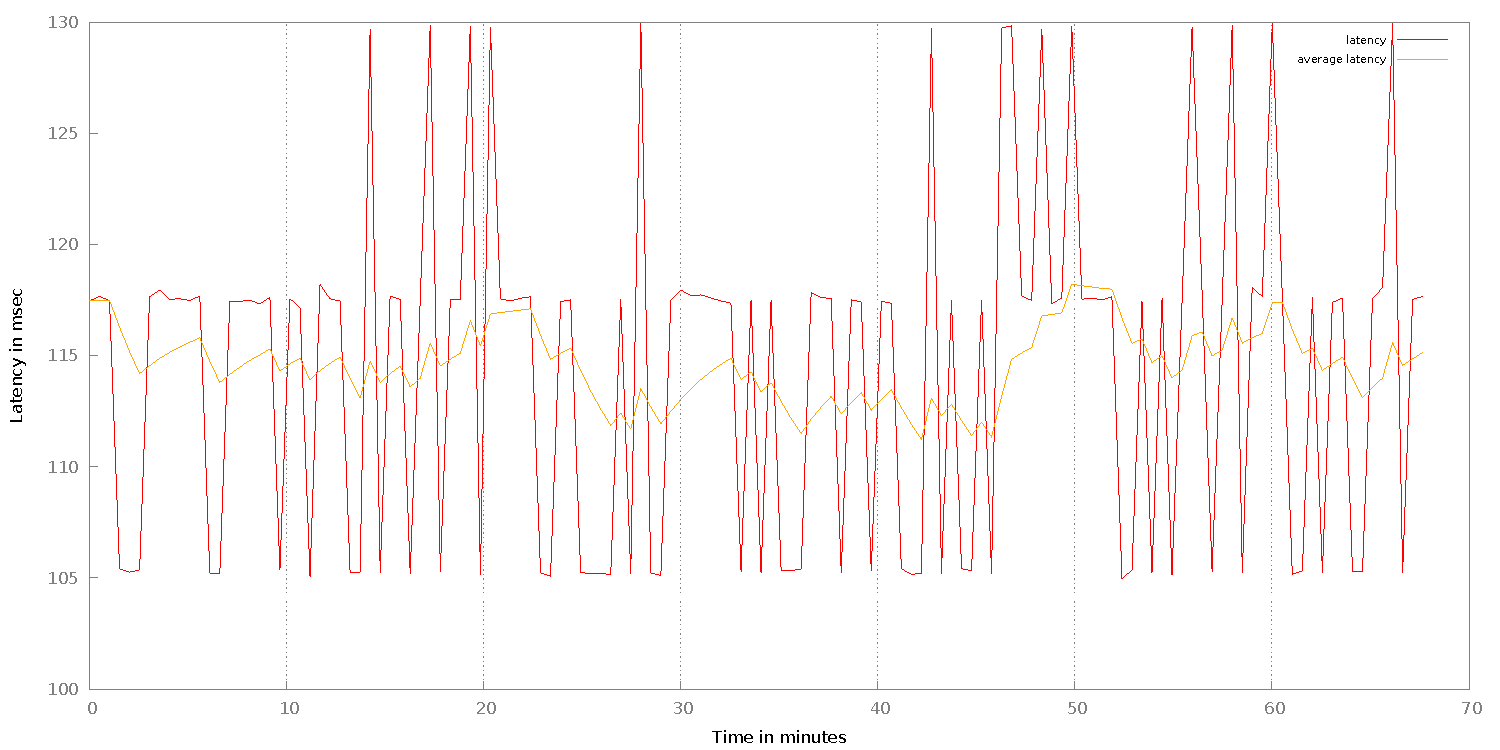
\includegraphics[width=\columnwidth]{latency_harvard_ethz.pdf}
\caption{Latency from Harvard to ETHZ}
\end{figure*}

\begin{figure*}[h!]
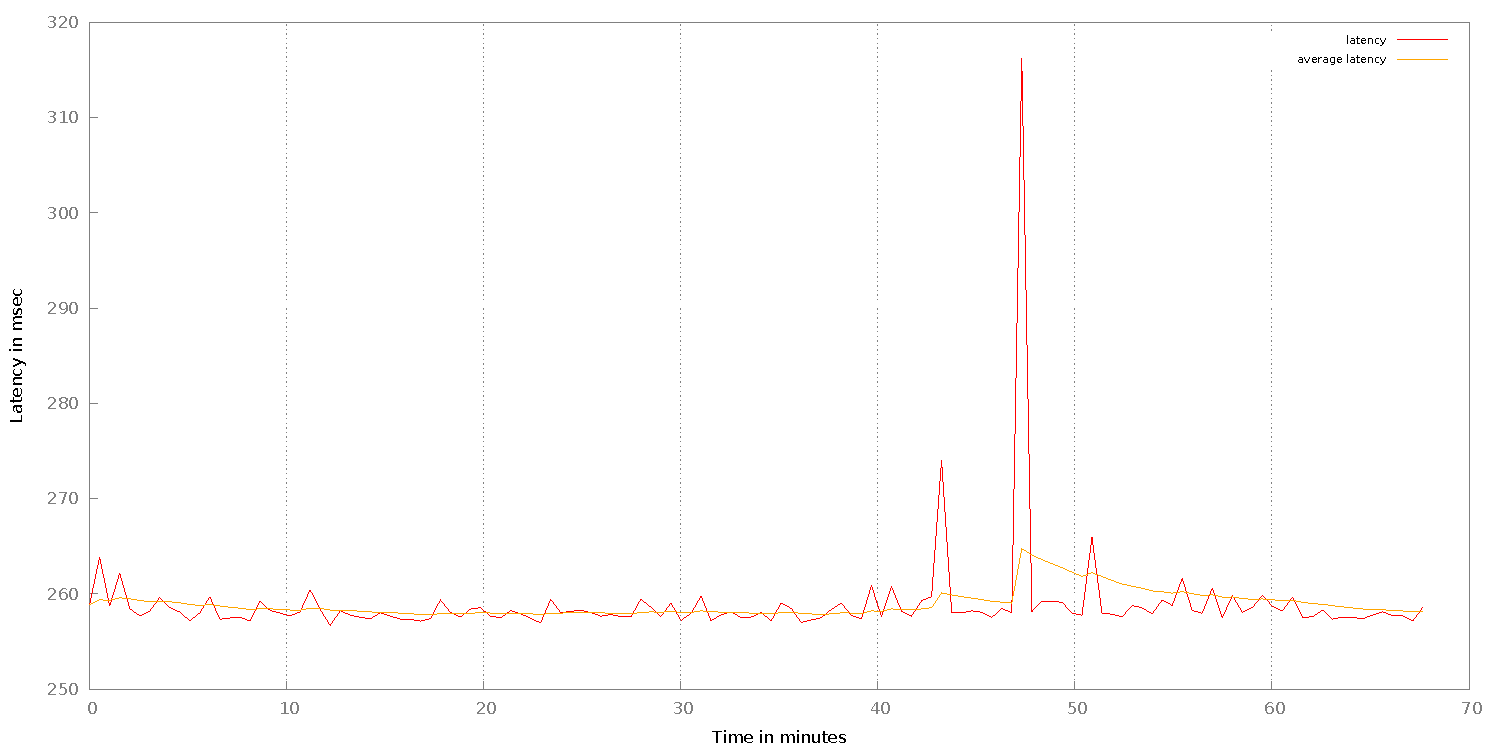
\includegraphics[width=\columnwidth]{latency_harvard_zhejiang.pdf}
\caption{Latency from Harvard to Zhejiang}
\end{figure*}

%\begin{figure*}[th]
% 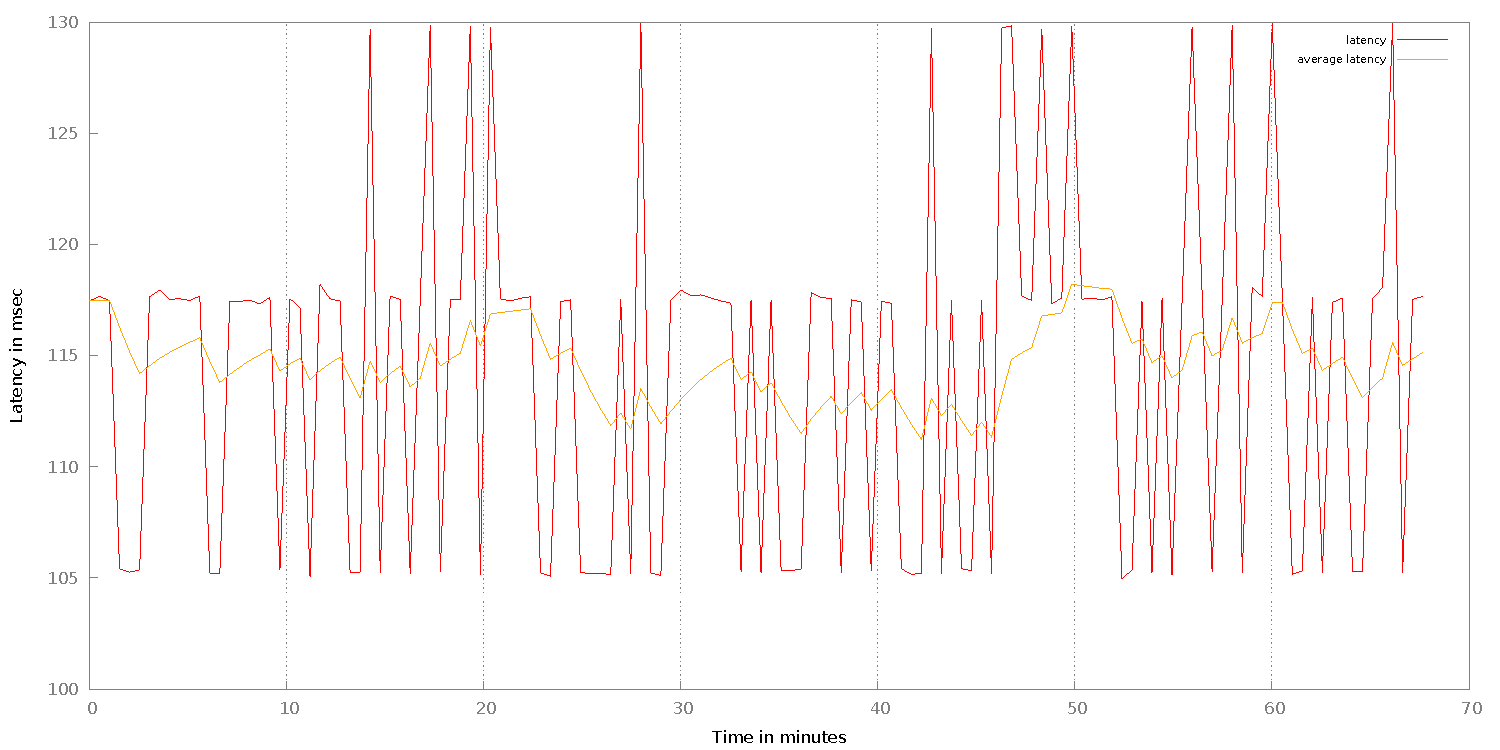
\includegraphics[width=\textwidth]{latency_harvard_ethz.pdf}
% \caption{Latency from Harvard to ETHZ}
% \label{fig:latency_harvard_ethz}
%\end{figure}
%----------------------------------------------------------------------------------------

\end{document}
